\documentclass[a4paper, 12pt]{article}

\usepackage[utf8]{inputenc}
\usepackage[T1, T2A]{fontenc}
\usepackage[english, russian]{babel}
\usepackage[top = 2cm, right = 2cm, left = 2cm, bottom = 2cm]{geometry}

\usepackage{amsmath} % \text{}
\usepackage{pgfplots} % for plot
\renewcommand{\arraystretch}{1.3} % for tables
\usepackage{indentfirst} % paragraph indentation
\usepackage{threeparttable}
\usepackage{multirow, array}
\usepackage{tikz}

% Change label separator
\usepackage{caption}
\captionsetup[table]{labelformat=simple, labelsep = endash, justification = raggedright, singlelinecheck = off, width = 0.75\textwidth}
\captionsetup[figure]{labelformat=simple, labelsep = endash, name = Рисунок}
\usepackage{pscyr}
\usepackage[final]{pdfpages}

\begin{document}
\section{Статический расчет и выбор элементов}
\subsection{Пьезоэлемент}
Рассчитаем пьезоэлемент, представленный на рисунке ниже. Частота собственных колебаний $f_0 = 1$ МГц. Материал ЦТС-19. \par 
\begin{figure}[h!]
	\begin{center}
	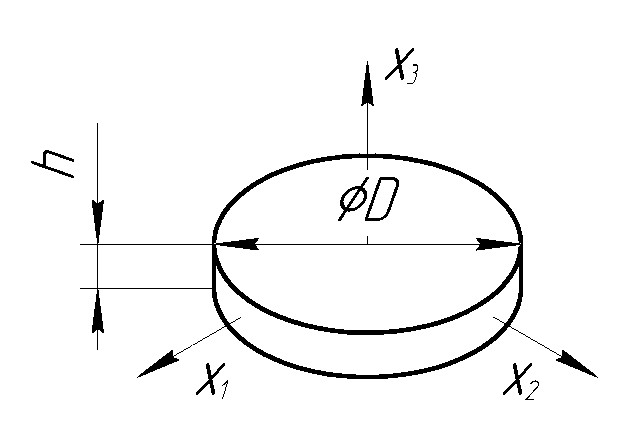
\includegraphics[width = 0.5\textwidth] {images/PiezoceramicScheme.pdf}
	\end{center}
	\caption{Пьезоэлектрик: h - ширина, D - диаметр}
\end{figure}
Для соблюдения резонансной частоты, необходимо, чтобы ширина пьезоэлемента была равна половине длинны волны. Из этого условия выведена формула для частоты собственных колебаний:
\begin{equation}
	f_0 = \frac{c}{2h}
\end{equation}
где $c$ - скорость звука в материале. По данной формуле можем найти ширину пьезоэлектрика:
\begin{equation}
	h = \frac{v_1}{2f_0} = \frac{3\cdot 10^3}{2\cdot10^6} = 0.0015 \text{ м} = 1.5\text{ мм}
\end{equation}

Теперь можем найти диаметр диска, для упрощения рассчетов, возьмем его на порядок больше толщины:
\begin{equation}
	D = 10h = 15 \text{ мм}
\end{equation}

Сформируем уравнения состяния нашего пьезоэлемента. Поскоьку $D \gg h$ мы можем пренебречь поперечными колебаниями, направленными вдоль $x_1$ и $x_2$ и рассматривать одномерную модель пьезоэлемента. В таком случае вся деформация происходит только в направлении оси $x_3$, вектор колебательной скорости и вектор напряженности электрического поля тоже направлены вдоль оси $x_3$. Учитывая эти обстоятельства запишем

\begin{align}
	& \rho\frac{\partial^2 u}{\partial t^2}  = \frac{\partial \sigma}{\partial x} \\
	& \sigma  = C_{33}\frac{\partial u}{\partial x} - e_{33}E\\
	& D  = \varepsilon_{33} E + e_{33}\frac{\partial u}{\partial x} \\
	& \frac{\partial D}{\partial x} = 0
\end{align}
где: $\rho$ - плотность [кг/м] \\ 
\hspace*{8mm} $v$ - скорость смещения точек среды (колебательная скорость) [м/с] \\
\hspace*{8mm} $\sigma$ - механическое напряжение [Па] \\
\hspace*{8mm} $C_{33}$ - коэффициент упругостьи [Па] \\
\hspace*{8mm} $e_{33}$ - пьезомодуль  [Кл/м$^2$] \\
\hspace*{8mm} $E$ - напряженность электрического поля [В/м] \\
\hspace*{8mm} $D$ - электрическое смещение [Кл/м$^2$] \\
\hspace*{8mm} $\varepsilon$ - абсолютная диэлектрическая проницаемость [Ф/м] \par 
\vspace{0.5cm}

Уравнение (25) представляет второй закон Ньютона для сплошной среды. Уравнение (26) дает описание обратного пьезоэффекта, т.е. возникновение механических напряжений и деформаций (колебаний среды) под действием электрического поля. Уравнение (27) формулирует прямой пьезоэффект – возникновение тока смещения и электрического поля в напряженно-деформированном теле. Уравнение (28) - это уравнение электрического баланса - оно указывает, что в материале отсутствуют объемные электрические заряды.
 


Пьезомодули $e_{33}$ и $d_{33}$ связаны между собой соотношением:
\begin{equation}
	e_{33} = C_{33} d_{33}
\end{equation}

Выразив из уравнения (27) напряженность $E$, подставим полученное выражение в (27) из корторого получим выражение для механического напряжения $\sigma$. Продифференцируем $\sigma$ по $x$ и подставим в (25), учитывая условие (28). В итоге получим дифференциальное уравнение в частных производных.

\begin{equation}
	\rho \frac{\partial^2 u}{\partial t^2} = \left( C_{33} + \frac{e_{33}^2}{\varepsilon_{33}} \right)\frac{\partial^2 u}{\partial x^2}
\end{equation}

Далее запишем соотношения для напряжения и тока пьезоэлемента. Очевидно, напряжение на контактах пьезопластины $U_\text{ПЭП}$ можно определить, интегрируя напряженность электрического по толщине пластины:

\begin{equation}
	U_\text{ПЭП} = \int_{0}^{h}{E dh} = E\cdot h
\end{equation}

Ток, протекающий через пьезоэлемент, равен	

\begin{equation}
 I_\text{ПЭП} = S_\text{ПЭП} \cdot i = \frac{\pi D^2}{4} \cdot i
\end{equation}
где $S_\text{ПЭП}$ - площать пластины, м$^2$.

Разложим подаваемое напряжение в ряд Фурье и оставим только первую гармонику. Она имеет вид: 
\begin{equation}
	U_\text{ПЭП} = U_m \sin{(\omega_0 t)}, \text{    } t \in [0, \tau]
\end{equation}
здесь $\omega_0 = 2 \pi f_0$ - круговая частота, $\tau = \displaystyle\frac{1}{2f_0}$ - длительность импульса, $U_m$ - амплитуда напряжения. Тогда можем найти значение частной производной напряженности по времени.
\begin{equation}
	\frac{\partial E}{\partial t} = U_m \omega \cos{(\omega_0 t)}
\end{equation}
\end{document}